% Notes on the writing of the Master Thesis
% Book: How to Write a Lot, Paul Silvia, 2nd Edition
% Book: Getting Things Done, David Allen
%
%
% Mögliche Abgrenzung von anderen: Den hybriden Ansatz von SBST mit DSE verwenden, 
% so wie im Paper von Baars et al.
%
% Mögliche weitere Evaluation: Vergleiche die Coverage von generierten Tests zu der 
% Coverage von manuell geschriebenen Tests von Entwicklern in evaluierten Programmen.
% 

\documentclass{article}
% Please do not change this options...
\usepackage[a4paper, total={6in, 10in}]{geometry}
\usepackage{graphicx}
\graphicspath{ {./img/} }
\usepackage{todonotes}
\usepackage{acronym}
\usepackage{algorithm}
\usepackage{amsmath}
\usepackage{algpseudocode}
\algblock{Input}{EndInput}
\algnotext{EndInput}
\algblock{Output}{EndOutput}
\algnotext{EndOutput}
\newcommand{\Desc}[2]{\State \makebox[2em][l]{#1}#2}
\usepackage[T1]{fontenc}
\makeatletter
\newcommand\BeraMonottfamily{%
  \def\fvm@Scale{0.85}% scales the font down
  \fontfamily{fvm}\selectfont% selects the Bera Mono font
}
\makeatother


\usepackage{listings,multicol}
\lstset{
  numbers=left,
  xleftmargin=2.5em,
  framexleftmargin=2.5em,
  frame=tb,
  stepnumber=1,    
  firstnumber=1,
  numberfirstline=true,
  basicstyle=\BeraMonottfamily,
  identifierstyle=,
  stringstyle=\ttfamily,
  %keywordstyle=\color{OliveGreen},
  keywordstyle=,
  showstringspaces=false
}

% This package must be declared last
\usepackage{cleveref}

\begin{document}

\title{Master Thesis}
\author{Vsevolod Tymofyeyev}
\date{\today}
\maketitle

\tableofcontents
\newpage
\section{Introduction}
In der Programiersprachenwelt, in der es zwei große Fronten gibt (low-level Sprachen, die auf Kosten von Sicherheit mehr Performanz bieten und high-level Sprachen, die durch bestimmte Konstrukte wie Garbage-Collector Sicherheiten für Programmierer bieten, die jedoch zu Laufzeit-Overhead führen) versucht Rust beides zu verbinden. Die statisch typisierte Sprache für Systemprogrammierung verspricht eine ähnlich hohe Performanz wie C++ mit erweiterter Typ- und Speichersicherheit by default. Invarianten werden zur Kompilierzeit sichergestellt, wodurch Abstraktionen (sogenannte Zero-Cost-Abstractions) und automatische Speicherverwaltung mit keinen Laufzeitkosten verbunden sind, wie es zum Beispiel bei Sprachen mit Garbage Collection der Fall ist. Rust verhindert unter anderem folgende oft verbreitete Probleme: dangling pointers, data races, integer overflow, buffer overflow, iterator invalidation. Nur die integer und  buffer overflows werden zur Laufzeit überprüft, wobei die buffer overflows durch das Benutzen von Iteratoren auf statische Checks reduziert werden können~\cite{Anderson2016}. Diese Symbiose führt dazu, dass die Sprache besonders attraktiv auf Entwickler wirkt, wodurch sie trotz ihres sehr jungen Geschichte bereits seit mehreren Jahren die Beliebtheitsrankings stürmt~\cite{StackOverflow2020}. Selbst Spitzenkonzerne erwägen die Anwendung von Rust in Teilen ihrer Software. Laut Microsoft und Google sind 70\% der in ihrer Software in den vergangenen Jahren gefundenen Fehler auf Speicherlecks zurückzuführen, hervorgerufen durch die weitverwendeten unsicheren Sprachen wie C und C++~\cite{Microsoft2019MemoryBugs, RustInAndroid}. Microsoft, SpaceX, Google, Amazon AWS und viele andere Unternehmen fingen bereits an, Rust in ihren Produkten zur erhöhten Sicherheit zu verwenden~\cite{MicrosoftJoinsRust, AmazonLovesRust, RustInAndroid, GoogleRustFoundation}.

Nichtsdestotrotz, kann auch der Rust Compiler nicht die komplette Korrektheit eines Programms garantieren, wodurch auch bei der Programmierung mit dieser Sprache das Testen der geschriebenen Software einem nicht erspart bleibt. Das Verhalten einer Software kann mit Hilfe von Tests überprüft werden, zum Beispiel Unit Tests, die kleinste Einheiten eines Programms, Units, isoliert ausführen. Software Testen erfodert jedoch Inputdaten, deren manuelle Selektion die Aufgabe eines Programmierers ist. Dieses Vorgehen ist aber in der Regel sehr aufwändig und kostenintensiv. Eine genügend komplexe Software kann Tausende Ausführungspfade haben, die durch verschiedene Inputdaten angesteuert werden und von einem Menschen leicht übersehen werden können. Schließlich müssten fast genauso viele Tests geschrieben werden. Ein weiterer Punkt ist, dass sich Software-Anforderungen mit der Zeit ändern können, was dazu führt, dass existierende Testsuites dadurch eventuell manuell verändert bzw. im schlimmsten Fall neu geschrieben werden müssen. Somit ist das Abdecken von allen möglichen Ausführungsfällen oder gar eine exhaustive Coverage schlicht wirtschaftlich und menschlich kaum zu leisten~\cite{Myers2012}. Es wird angenommen, dass ungefähr die Hälfte des Budgets in Software Projekten für das Testen ausgegeben wird~\cite{Beizer2003}. Außerdem, trotz der ausgereiften Testing Tools, stehen Entwickler oft unter Zeitdruck (z. B. Deadlines bei Projekten) und haben nicht genug Zeit, die immer komplexer werdende Software zu testen. Das ist ein großes Problem, denn auch wenn einige kleinen Bugs nur zur Unzufriedenheit eines Endnutzers führen, können einige andere erhebliche wirtschaftliche und selbst gesundheitliche Schäden auslösen~\cite{Myers2012}. \todo{Ein paar Beispiele für krasse Vorfälle wegen Software Bugs wären hier praktisch, z. B. Arianne V Explosion} Aus diesem Grund sind in den letzten Jahren bzw. Jahrzehnten viele Ansätze entstanden, um diesen Prozess zu automatisieren, indem Tests aus einer gegebenen Software generiert werden~\cite{McMinn_2004}. 

Alle möglichen Kombinationen von Inputdaten eines Programms zu testen ist jedoch auch automatisiert meistens nicht möglich und würde im Großteil der Fälle zu equivalenten Tests führen, die immer wieder das gleiche tun. Um den Aufwand zu vermeiden, versucht man, nur repräsentative Inputdaten für die jeweilige Equivalenzklassen zu finden, um Pfade, die von bestimmten Klassen von Inputdaten bestimmt werden, möglichst wenig ausführen zu müssen. Für diesen Zweck wird von vielen Tools symbolische Ausführung angewendet. Dabei wird das \ac{SUT} analysiert und symbolisch ausgeführt. Es wird eine von Constraints für die Inputdaten definiert, die nötig sind, um ein bestimmtes Ziel im ausgeführten Code zu erreichen~\cite{Clarke1976}. Praktisch bedeutet eine symbolische Ausführung jedoch viele komplexe algebraische Manipulationen, vor allem wenn es um Objekt-orientierte Container geht~\cite{Korel1990}. \ac{SBST} ist ein alternatives und sehr aktives Forschungsfeld, dessen Hauptidee ist, mit Hilfe metaheuristischer Suchtechniken eine begrenzte Anzahl von Tests innerhalb einer akzeptierbarer Zeit zu generieren, die ein möglichst hohes Testkriterium (z. B. Code Coverage) erfüllen~\cite{McMinn_2004}. 

Da Rust als stabile Programmiersprache als jung gilt und im Jahr 2015 in der Version 1.0 erschien~\cite{Rust10}, gibt es zum Stand des Schreibens nur relativ wenige Optionen für eine automatische Testgenerierung. Diese beschränken sich auf Tools, die mittels Symbolic Execution die möglichen Pfade in einem gegebenen Programm durchsuchen~\cite{cadar2008klee}. \todo{Weitere Tools?} Außerdem benutzen die Tools die IR von LLVM, welches vom Rust Compiler eingesetzt wird. Zusätzlich bringt das affine Typ-System von Rust~\cite{Anderson2016} einige Hürden mit, verglichen zu Sprachen wie z. B. Java. Es gibt aber zum Stand des Schreibens keinen bekannten Einsatz von \ac{SBST} für Rust. \ac{SBST} ist eine Kombination aus automatischer Testgenerierung und metaheuristischen Suchtechniken. Diese Unterkategorie von SBSE greift zu Optimisierungsalgorithmen, um ein eigentlich NP-hartes Problem der Testgenerierung mit möglichst hoher Testabdeckung möglichst effizient und effektiv zu lösen~\cite{Khari2019}. SBST optimizes a solution as much as possible with respect to a certain objective, which could be test case priorization, test suite minimization, max out real-time properites of the SUT, and so on~\cite{Khari2019}. Die dadurch generierten Tests streben eine höhere Coverage an, um möglichst viele Fälle abzudecken. 

\section{Background}
\subsection{Test Generation in General}
\todo{Structural, functional, etc. testing}
Testsgenerierung ist ein aktiv erforschtes Feld in der Wissenschaft. Im Idealfall kann für ein Programm eine Testsuite von Unit Tests generiert werden, die alle möglichen Pfade im \ac{SUT} abdecken und gleichzeitig die Korrektheit der Ausführung jedes einzelnen Pfades durch automatische Orakel überprüft, beispielsweise durch Assertions. Ein Orakel ist ein Mechanismus zum Überprüfen, ob ein Output bei einem gegebenen Input richtig ist, beispielsweise mit Hilfe einer formalen Spezifikation~\cite{McMinn2009}. Leider ist das oft nicht möglich. Zum einen können in einem Programm Ausführungspfade existieren, die schlicht unter keinen Umständen erreicht werden können. Zum anderen hat Software nur sehr selten eine formale Spezifikation, die bei der Generierung verwendet werden kann, um Orakel zu generieren. Somit muss in den meisten Fällen ein Entwickler bzw. Tester die generierte Testsuite manuell mit Orakeln versehen (dazu muss er/sie natürlich selbst wissen was das richtige Verhalten ist)~\cite{Fraser_2013}. Dazu muss die generierte Testsuite aber auch möglichst klein und für den Menschen verständlich gehalten werden. 

Bei einer Testgenerierung wird das Coverage-Kriterium oft als eine Leitlinie benutzt~\cite{Fraser_2011}. Ein Coverage-Kriterium ist eine Sammlung von Test-Zielen, die typischerweise eins nach dem anderen abgearbeitet bzw. abgedeckt werden, wobei die notwendigen Input-Daten beispielsweise symbolisch oder such-basiert ermittelt werden. Eine beliebte Art des Coverage-Kriteriums ist die Branch-Coverage. 

Branches sind z. B. Arme einer if-Verzweigung oder eines Schleifenkopfes. Diese werden dann ausgeführt, wenn ein bestimmter boolischer Ausdruck zu \lstinline{true} bzw. \lstinline{false} evaluiert. Branches können auch verschachtelt sein, und um passende Werte zu finden, um einen (verschachtelten) Branch zu erreichen, kann symbolic execution bzw. seine dynamische Erweiterung mit konkreten Werten verwendet werden. Dabei wird ein Pfad aufgebaut, der mit einem \ac{SMT}-Solver nach konkreten Werten (falls solche existieren und der Pfad überhaupt erreichbar ist) aufgelöst werden kann. Eine Alternative zur symbolischen Ausführung ist eine meta-heuristische Suche. Fraser und Arcuri~\cite{Fraser_2011} listen ein paar verwante Paper dazu auf. 

\subsection{Automatically Generated Oracles}
\label{sec:generated-oracles}
Davis and Weyuker~\cite{10.1145/800175.809889} haben den Begriff non-testable programs einfegührt, der solche Programme einschließt, für die es keinen Testorakel gibt oder ein Testorakel praktisch nicht umsetzbar ist, und man somit das Ergebnis der Berechnung nicht auf Korrektheit überprüfen kann. Dazu gehören Programme, die entweder erstellt wurden, um das Ergbenis überhaupt zu erfahren, oder Programme, die zu viele Ergebnisse liefern, um sie alle zu überprüfen, oder der Entwickler hatte die Spezifikation missverstanden. Um das Problem eines fehlenden Orakels zu lösen, führten die Autoren einen sogenannten Pseudoorakel ein. Ein Pseudoorakel ist ein zweites, unabhängig implementiertes Programm, das derselben Spezifikation entsprechen muss. Es ist wichtig, dass die zwei Programme von separaten Teams ohne Zwischenkommunikation erstellt werden, damit keine Missverständnisse von einem in das andere Team propagieren können. Anschließend können die Ergebnisse der Berechnungen des originalen Programms und des Pseudoorakels verglichen und es kann über die Validität entschieden werden. 

Das manuelle Erstellen von Pseudoorakeln ist sehr mühselig und ist im Kontext von Testgenerierung für große Projekte nicht lohnenswert. Harman et al.~\cite{Harman2004} haben das Prinzip der Testability Transformations vorgestellt. Diese sind Quelltext-zu-Quelltext Transformationen, die zum Verbessern der Performanz verschiedener Testgenerierungstechniken führen sollen. McMinn~\cite{McMinn2009} hat diese Idee aufgegriffen und vorgeschlagen, Pseudoorakel für ein gegebenes Programm automatish zu generieren. Er wendet Testability Transformations an, um das originale Programm zu verändern und eine zweite Version zu generieren, die scheinbar gleiche Ausgaben wie die originale haben sollte, es jedoch zu Diskrepanzen kommen kann. Dazu hat er zwei Beispiele aufgeführt: Fließkomma-Arithmetik und Multithreading in Java. Beim Ersteren werden, beispielsweise Additionen zwischen primitiven Fließkommatypen, die nach dem IEEE-Standard etwas ungenau in den hinteren Nachkommastellen sind~\cite{10.1145/103162.103163}, durch Javas BigDecimal vertauscht. Zum Beispiel führt die Berechnung~$0.1 + 0.1 + 0.1$ in Java zum Ergebnis~$0.30000000000000004$, anstatt~$0.3$ (siehe~\cref{lst:java-transformations}).

\begin{lstlisting}[language=Java, caption=Comparing floating-point arithmetic in Java using double compared to BigDecimal~\cite{McMinn2009}, label=lst:java-transformations]
System.out.println(0.1 + 0.1 + 0.1);
// Ausgabe: 0.30000000000000004

System.out.println(
    new BigDecimal("0.1").add(
        new BigDecimal("0.1").add(
            new BigDecimal("0.1")
        )
    )
);
// Ausgabe: 0.3
\end{lstlisting}
In einem anderen Beispiel wendet McMinn Transformationen zum Serialisieren/Deserialisieren eines Multithreading-Programm. Dabei werden Methoden einer Klasse mit Javas \lstinline{synchronize} versehen bzw. das Schlüsselwort wird bei bereits synchronisierten Methoden entfernt. \lstinline{synchronize} sorgt dafür, dass nur ein Thread gleichzeitig die jeweilige Methode verwenden darf. In der Evaluation versucht der Autor, die durch Transformationen generierten Orakel mit Hilfe für eine genetisch-basierte Suche nach Input-Daten zu verwenden, die die Diskrepanz zwischen den Ausgaben eines originalen Programms und seines Psudoorakels maximieren. Damit können nicht nur potenzielle Bugs automatisch entdeckt (Diskrepanz), sondern auch ihr Schweregrad gemessen (Größe der Diskrepanz) werden. Die Idee von automataisch generierten Pseudoorakel wurde auch von Fraser und Arkuri~\cite{Fraser_2013} aufgegriffen. \todo{Da fehlt was}

\subsection{Random Search}
Random Search ist eine Baseline Strategie, die nicht auf Rekombination, Mutation oder Selektion zurückgreift, sondern auf Ersetzen von bestehenden Lösungen setzt. Die Idee ist, immer wieder neue Lösungen aus dem Suchraum nach dem Zufallsprinzip zu sampeln, wobei eine vorige Lösung durch die neue ersetzt wird, falls der Fitnesswert der neuen Lösung besser ist. Random Search kann von einem Archiv Gebrauch machen, indem eine Samplingstrategie wie \todo{Samplingstrategie beschreiben} eingesetzt wird~\cite{Campos2017}.

Random Testing ist eine Variante von Random Search, die Test Suites inkrementell aufbaut. Mit Random Testing wird das Programm mit zufälligen Eingaben ausgeführt und die ausgeführten Strukturen des Programms werden beobachtet. Einzelne Test Cases werden aus dem Suchraum gesampelt, und falls ein Test Case die gesamte Coverage der Testsuite erhöht, wird er behalten und ansonsten verworfen~\cite{Campos2017}. Da die Landschaft der Fitnesswerte bei der Generierung von Unit Tests ziemlich flach ist und das ein relativ simples Suchproblem ist, kann Random Search mindestens genauso effektiv sein wie evolutionäre Algorithmen und manchmal sogar besser~\cite{Shamshiri2015a}. 

\subsection{Symbolic Execution}
Symbolische Ausführung ist keine Ausführung des Programms in direktem Sinne. Vielmehr ist das ein Prozess, bei dem Programmvariablen symbolische Ausdrücke zugewiesen werden, während ein Pfad in der Programmstruktur verfolgt wird~\cite{McMinn_2004}. So ein Pfad kann aus mehreren Einschränkungen bestehen. Symbolische Ausführung ist ein verbreiteter Ansatz, um Inputdaten oder ganze Unit-Tests zu generieren, indem die Pfadeinschränkungen aufgelöst werden. \todo{Werke über DS referenzieren} Grundsätzlich folgen alle Tools dem gleichen Prinzip: Statt Programme mit manuellen oder generierten Inputdaten laufen zu lassen, werden Inputdaten mit symbolischen Werten besetzt, die initial ''alles'' sein können~\cite{cadar2008klee}. Konkrete Operationen auf Daten werden durch solchen ersetzt, die die symbolischen Daten manipulieren können. Wenn sich die Ausführung des Programms verzweigt, behalten die Tools die Ausführung beider Branches ''im Auge''. Für jeden Branch wird eine Sammlung von Einschränkungen (Constraints) gespeichert, die für die Ausführung des jeweiligen Pfades gelten müssen. Wenn die Ausführung in einem Pfad endet oder das Programm abstürzt, kann daraus ein Test generiert werden, indem konkrete Werte als Inputdaten eingesetzt werden, die die entsprechenden Pfad-Constraints erfüllen. Wenn das Programm deterministisch und unverändert bleibt, führt eine Ausführung mit konkreten Inputdaten zum selbem Bug im Program. 

Dynamische symbolische Ausführung ist eine Erweiterung von symbolischer Ausführung, die erlaubt, mit Hilfe einer Kombination aus konkreten und symbolischen Werten eine Reihe von Problemen zu überwinden~\cite{Fraser_2013}. Es gibt eine Reihe von Tools, die für eine automatische Generierung von Tests auf DSE setzen, zum Beispiel CUTE and jCUTE~\cite{Sen2006} und KLEE~\cite{cadar2008klee}. KLEE hat zwei Ziele: (1) das Tool versucht, jede ausführbare Zeile in einem Programm auszuführen, d. h. hohe Statement Coverage zu erreichen und (2) bei jeder gefährlichen Operation (z. B. dereference, assertion) wird versucht zu überprüfen, ob es Werte gibt, die dabei zu einem Fehler führen könnten. Das letztere wird durch symbolische Ausführung erreicht. Da selbst in einfachen Programmen die Anzahl von Ausführungszuständen / -pfaden explodieren kann, wird von KLEE eine Reihe von Heuristiken und Optimisierungstechniken angewendet, um die Performanz zu erhöhen. Zum Beispiel werden nicht ganze Bäume bei Verzweigungen gecloned (Zustände sind nämlich Bäume), sondern es wird der write-on-copy Ansatz auf Objekt-Level angewendet. Unveränderte Teilbäume können von mehreren verschiedenen Zuständen referenziert werden. Außerdem wird versucht, Anfragen an den SAT Solver, um symbolische Werte in konkrete umzuwandeln, so weit vereinfacht wie möglich, da die Verarbeitungszeit der Anfragen alles andere dominiert. Auf diese Weise konnten die Autoren die Ausführungszeit des Tools auf den GNU Coreutils um das 15-fache beschleunigen.

\subsection{Evolutionary algorithms}
Der potenzielle Suchraum für mögliche Inputdaten selbst bei einem sehr simplen Programm kann unendlich groß sein. Metaheuristische Ansätze versprechen eine Abhilfe. Das sind keine geschlossenen Algorithmen an sich, sondern Strategien, die auf spezifische Probleme angepasst werden können. Für die Generierung von Testdaten wird eine problem-spezifische Fitnessfunktion definiert, mit deren Hilfe die Qualität möglicher Lösungen des Problems verglichen werden kann~\cite{McMinn_2004}. Metaheurische Suche wird nicht nur für Testdatengenerierung verwendet. Andere Verwendungen umfassen:
\begin{itemize}
	\item Coverage der Programmstruktur als Teil einer White-Box Teststrategie,
	\item das Auswerten eines spezifischen Programmfeatures nach seiner formalen Spezifikation,
	\item Versuche, automatisch Fehlerbedingungen oder Brüche von Assertions in einem Programm herbeizurufen
	\item Verifizierung nicht-funktionaler Features, beispielsweise worst-case Ausführungszeit eines Programmteils finden.
\end{itemize}
Evolutionary algorithms setzen auf simulierte Evolution bei der Suche nach Lösungen zu einem spezifischen Problem und evolvieren Lösungskandidaten mit Hilfe von speziellen Operatoren, die von Genetik und natürlicher Selektion inspiriert sind. Genetische Algorithmen sind die bekannteste Ausprägung der evolutionären Algorithmen und nehmen ihre Anfänge irgendwo her. \todo{Keine Ahnung, ob das überhaupt sinnvoll ist, die Geschichte davon aufzuschreiben.} Eine Suche mit genetischen Algorithmen wird auf Basis von Rekombination von Zwischenlösungen durchgeführt, einem Mechanismus, um Informationen zwischen Lösungen auszutauschen und somit neue züchten~\cite{McMinn_2004}.

\subsubsection{Genetic Algorithms}
McMinn hat ein super Beschreibung von genetischen und evolutionären Algorithmen, Selektion, Crossover, Mutation, fortgeschrittene Repräsentationen von Individuen~\cite{McMinn_2004}. Außerdem wird der genetische Algorithmus in \cite{Fraser2011} und \cite{Fraser_2013} beschrieben. \cite{Fraser_2013} beschreibt außerdem die Suchoperatoren. 

In seinem Paper beschreibt Harman~\cite{Harman2002}, wie bestimmte Variablen innerhalb von Verzweigungsknoten bei der Suche rausgefiltert werden können, weil sie keinen Einfluss auf die Branch Distance haben. Somit wird der Suchraum verkleinert. 

Genetische Algorithmen sind die meist verbreitete Form von evolutionären Algorithmen, da sie einfach zu implementieren sind und im Schnitt gute Ergebnisse erzielen. Der Name ''genetischer Algorithmus'' kommt von der Analogie zwischen dem Enkodieren eines Lösungskandidaten als eine Sequenz von simplen Komponenten und der genetischen Struktur eines Chromosomes. Diese Analogie wird fortgeführt, indem einzelne Lösungen als Individuen oder Chromosomen bezeichnet werden~\cite{Campos2017}. Demnach werden Komponenten einer Lösung Gene genannt, wobei mögliche Werte einer Komponente Alleles und ihre Position in der Sequenz Locus heißen. Des Weiteren wird eine tatsächliche enkodierte Repräsentation einer Lösung, die von einem genetischen Algorithmus manipuliert wird, Genotyp und eine dekodierte - Phenotyp genannt~\cite{McMinn_2004}. Algorithm~\labelcref{alg:genetic-algorithm} zeigt abstrakt die Funktionsweise eines Standard genetischen Algorithmus. Die initiale Population wird typischerweise zufällig generiert oder aus einem bestimmten Seed generiert. In folgenden Generationen werden Nachkommen mittels Optimisierungs- oder Suchoperatoren gezüchtet, also Rekombination und Mutation. Es gibt viele Variationen des Standard GA. Zum Beispiel werden bei der monotonen Variante des Standard GA nach der Mutation und Evaluation der Fitness der Nachkommen entweder die besten Nachkommen oder die besten ''Parents'' der nächsten Population hinzugefügt. Beim Standard GA werden an der Stelle sowohl ''Parents'' als auch Nachkommen der nächsten Population hinzugefügt. Eine weitere Variante von Standard GA ist der Steady State GA, der wie die monotone Variante nur die besten Individuen nach einer Mutation behält, jedoch anstatt eine neue Population von Nachkommen zu kreieren, ersetzt die ''Parents'' durch Nachkommen in der ursprünglichen Population~\cite{Campos2017}. 

Die unter anderem wesentlichen Punkte beim Algorithm~\labelcref{alg:genetic-algorithm} sind das Messen der Fitness eines einzelnen Tests und der Mutationsoperator oder -funktion. Diese sind Faktoren, mit deren Hilfe eine aktuelle Population zu einer neuen evolviert werden, die mehr Chancen hat, einen Target abzudecken. Die Fitness bestimmt eines Individuums, zu überleben und in der neuen Population, evtl. in einer mutierten Form, teilzunehmen. Ein Mutationsoperator bestimmt hingegen, auf welche Weise neue Individuen (Test Cases) aus gegebenen generiert werden~\cite{Tonella2004}. Die Selektion von Individuen wird durch Fitness Funktionen gesteuert, sodass Individuen mit guter Fitness mit höher Wahrscheinlichkeit überleben und in der Zucht von Nachkommen teilnehmen. Im Kontext von Testgenerierung basieren Fitness Funktionen auf Kriterien der Code Coverage, wie z. B. Statement oder Branch Coverage. In den letzten Jahren gab es einen Trend, die Suche nach mehreren Coverage Kriterien gleichzeitig zu optimieren. Da Coverage Kriterien typischerweise keine widersprüchliche Ziele darstellen, können diese in einer weigted linearen Funktion kombiniert werden~\cite{Rojas2015}. Eine hohe Anzahl von Coverage Zielen kann jedoch die Performanz eines evolutionären Algorithmus negativ beeinflussen. Um das zu vermeiden, können generierte Tests für abgedeckte Ziele in einem Archiv gespeichert werden~\cite{Rojas2017}, wobei die Fitness Funktion dynamisch adaptiert wird, um die Suche nur in Richtung nicht abgedeckter Ziele zu leiten. Der Archiv kann auch bei für bessere Effektivität von Suchoperatoren verwendet werden, in dem beispielsweise neue Tests durch Mutation von bestehenden aus dem Archiv und nicht zufällig generiert werden~\cite{Campos2017}. 
\begin{algorithm}
\caption{A high level description of a standard genetic algorithm~\cite{Campos2017}}\label{alg:genetic-algorithm}
\begin{algorithmic}
\Input
  \Desc{$C$}{Stopping condition}
  \Desc{$\delta$}{Fitness function}
  \Desc{$p_s$}{Population size}
  \Desc{$s_f$}{Selection function}
  \Desc{$c_f$}{Crossover function}
  \Desc{$c_p$}{Crossover probability}
  \Desc{$m_f$}{Mutation function}
  \Desc{$m_p$}{Mutation probability}
  \EndInput
  \Output
  \Desc{$P$}{Population of optimized individuals}
  \EndOutput
\State $P \gets GenerateRandomPopulation(p_s)$
\State $PerformFitnessEvaluation(\delta, P)$

\While{$\neg C$}
    \State $N_P \gets \{\}$
    \While{$\left| N_P \right| < p_s$}
        \State $p_1, p_2 \gets Selection(s_f, P)$
        \State $o_1, o_2 \gets Crossover(c_s, c_p, p_1, p_2)$
        \State $Mutation(m_f, m_p, o_1)$
        \State $Mutation(m_f, m_p, o_2)$
        \State $N_P \gets N_P \cup \{o_1, o_2\}$
    \EndWhile
    \State $P \gets N_P$
    \State $PerformFitnessEvaluation(\delta, P)$
\EndWhile
\State \Return $P$
\end{algorithmic}
\end{algorithm}

\subsubsection{Crossover}
\label{sec:background-crossover}
Ein wesentlicher Teil von genetischen Algorithmen ist die sogenannte Rekombination oder auch Crossover. Dieser Operator nimmt zwei Parent-Lösungen als Input und verbindet sie in einer bestimmten Weise, um zwei Nachkommen-Lösungen zu produzieren. Es gibt viele verschiedene Arten von Rekombination, aber die einfachste ist die One-Point-Rekombination~\cite{McMinn_2004}. Dabei wird ein einzelner Punkt in den zwei Lösungssequenzen gewählt, der die Sequenzen in Kopf und Schwanz trennt. Die Köpfe bzw. die Schwänze werden dann zwischen den beiden Sequenzen ausgetauscht. Eine One-Point Rekombination von zwei Individuen $[0, 255, 0]$ und $[255, 0, 255]$, die in Binärform jeweils als $000000001111111100000000$ und $111111110000000011111111$ enkodiert wären, an der Stelle $12$ würde zu folgenden zwei Nachkommen führen~\cite{McMinn_2004}:
\[
\left.\begin{array}{c}
000000001111 \\  %  
111111110000 % 
\end{array}\right| 
\begin{array}{c}
111100000000 \\  %  
000011111111 % 
\end{array} \longrightarrow
\begin{array}{c}
000000001111000011111111 \\  %  
111111110000111100000000 % 
\end{array}
\]
\todo{Es gibt auch viele andere Rekombinationsverfahren, die man hier evtl. anführen könnte}


\subsubsection{Selection}
Es können viele verschiedene Selektionsmechanismen angewendet werden, um zu entscheiden, welche Individuen für eine Nachkommenschaft herangezogen werden sollen. Der Fokus liegt dabei auf der Fitness der Individuen. Der Fitnesswert kann dabei entweder direkt verwendet oder erst auf eine bestimmte Weise skaliert werden. 

Genetische Algorithmen speichern eine ganze Population von Lösungen, statt nur einer aktuellen Lösung. Das hilft vor allem initial mehr vom Suchraum zu sampeln, indem mehrere Startpunkte definiert werden. Die Population wird iterativ rekombiniert und mutiert, um weitere Populationen durch das Evolvieren zu züchten, die als Generationen bekannt sind. Die Idee einer Rekombination besteht darin, fittere Individuen vorzuziehen, in der Hoffnung, dadurch auch fittere Nachkommen zu züchten. Jedoch kann eine viel zu sehr fokusierte Selektion auf am meisten fitte Individuen dazu führen, dass diese die die nächsten Generationen dominieren werden und so aufgrund niederiger Diversität die Suche nur auf einen bestimmten Bereich im Suchraum begrenzen. Auf der anderen Hand, eine zu schwache Selektion kann dazu führen, dass die Suche in einer viel zu breiten Exploration des Suchraumes endet, wodurch kein signifikanter Fortschritt in Richtung optimaler Lösung geschafft wird~\cite{McMinn_2004}. 

Der originale Selektionsalgorithmus von Holland \todo{Zitat einfügen: Holland JH. Adaptation in Natural and Artificial Systems. University of Michigan Press: Ann Arbor, MI, 1975.} setzte auf \textit{Fitness-proportionale Selektion}. Dieser Selektionsmechanismus wies jedem Individuum, wie oft es für Reproduktion ausgewählt wird, basierend auf der Fitness des jeweiligen Individuums im Vergleich zum Rest der Population. Der Prozess ist analog zu einer Roulettescheibe: Jedem Individuum wird ein Abschnitt auf der Scheibe entsprechend seinem Fitnesswert zugewiesen. Die Scheibe wird dann $N$ mal gedreht, um $N$ ''Eltern'' auszuwählen. Am ende jeder Runde bestimmt die Position des Markers auf der Scheibe das Individuum, das als ''Parent'' für die nächste Generation ausgewählt wurde. Fitness-proportionale Selektion kann aber zu Schwierigkeiten führen, eine konstante Selection Pressure zu halten. Selection Pressure ist die Wahrscheinlichkeit, dass das beste Individuum ausgewählt wird im Vergleich zur durchschnittlichen Wahrscheinlichkeit aller Individuen, ausgewählt zu werden. In den ersten Generationen einer Suche die Varianz von Fitnesswerten einer Population ist typischerweise hoch, was dazu führt, dass auch die Selection Pressure einer Fitness-proportionalen Selektion hoch ist. Das kann zu einer viel zu früher Konvergenz führen. In den späteren Generationen, wenn sich die Fitnesswerte von Individuen nicht mehr so stark unterscheiden, fällt die Selection Pressure ab, was zur Stagnation bei der Suche führen kann. 

Sobald die Sammlung von ''Parents'' ausgewählt wurde, wird die Rekombination angewendet, um die nächste Generation zu züchten. Crossover wird auf die ausgewählten Individuen mit der Wahrscheinlichkeit $p_c$ angewendet. $p_c$ wird auch als Crossover rate oder Crossover probability bezeichnet. Falls Crossover angewendet wird, werden die neuen Nachkommen der neuen Population hinzugefügt. Ansonsten werden die selektierten ''Parents'' unverändert in die neue Population kopiert. Nach diesem Schritt wird die Mutationsphase eingeleitet, die für das Einführen bzw. Wiedereinführen eines neuen genetischen ''Materials'' verantwortlich ist, welcher Diversität der Suche erhöhen soll. 

\textit{Lineares Ranking} von Individuen ist eine Technik, die dieses Problem überwinden kann. Dabei werden Individuen nach ihrer Fitness sortiert, wobei die besten Individuen nach ihrem Rank ausgewählt werden~\cite{whitley1989genitor}. \todo{Irgendwie nicht ganz verständlich. Näheres unter der Quelle nachzulesen}

\textit{Tournament Selection} ist ein noisy, aber schnelles Verfahren, um Nachkommen auszuwählen. Die Population muss dabei nicht nach der Fitness sortiert sein. Zwei Individuen werden zufällig aus der Population ausgewählt. Dann wird eine eine zufällige reale Zahl $0 < r < 1$ gezogen. Wenn $r$ kleiner als $p$ (wobei $p$ die Wahrscheinlichkeit ist, dass das fittere Individuum ausgewählt wird) ist, gewinnt das Individuum mit der besseren Fitness und wird als ''Parent'' für die nächste Generation ausgewählt, ansonsten wird das andere Individuum ausgewählt. Danach werden die beiden Individuen zurück in die Population ''gelegt'', um bei der nächsten Runde wieder gewählt werden zu können. Diese Prozedur wird $N$ mal wiederholt, bis die erforderliche Anzahl von ''Parents'' für die nächste Generation ausgewählt wird. 


\subsection{Mutation}

\subsubsection{Advanced Individual Encoding}
In einfachen Algorithmen werden Individuen typischerweise im Binärformat enkodiert. Das bringt aber einige Schwierigkeiten mit sich, vor allem wird dabei oft das Konzept verletzt, dass eine Nachbarslösung mit einer einfachen Mutation zu bewerkstelligen sein sollte. Das ist aber zum Beispiel wäre die Integerzahl 7 in der Binärrepräsentation als $0111$ enkodiert, die 8 aber als $1000$. Das heißt, um die Nachbarslösung von 7, also die 8, zu erreichen, müssten die verwendeten Suchoperatoren alle vier Bits verändern. Eine Binärrepräsentation der Lösung hat zwar den Effekt, dass die Lösungssequenz aus kleinsten Komponenten (Bits) besteht, die zu effektivsten Ergebnissen von Rekombination und Mutation führen. Davis~\cite{Davis1991} zeigte jedoch in seinen Experimenten mit genetischen Algorithmen, dass echte Lösungsrepräsentationen besser abgeschnitten hatten, als Binärrepräsentationen. Die Verwendung von echten Lösungsrepräsentationen stellt aber die Frage, wie die Rekombinations- und Mutationsoperatoren implementiert werden sollen. Die Rekombination braucht im Grunde nur die Repräsentation der Sequenz von Komponenten einer Lösung und kann ähnlich angewendet, wie auf eine Binärrepräsentation. Der Mutationsoperator muss dagegen auf jeden Fall auf das spezifische Problem zugeschnitten sein, z. B. kann eine Integerzahl trivialerweise durch eine zufällige ersetzt werden. In einer fortgeschrittenerer Mutation könnte eine solche Integerzahl leicht verändert werden, indem ein kleiner Betrag hinzu addiert bzw. subtrahiert wird. Auf diese Weise wird auch das Prinzip der lokalen Suche beibehalten~\cite{Davis1991}. 


\subsubsection{Objectives}
Generell greifen such-basierte Techniken oft zu solchen Coverage-Kriterien wie Branch Coverage, Statement Coverage oder Mutation Coverage, die eine numerische Angabe sind, wie gut eine Testsuite ist. Eine Testsuite besteht aus einzelnen Tests, wobei ein Test nichts anderes als eine Sequenz von Statements variabler Länge ist. Beim \ac{WS} Ansatz misst die gewählte Fitness Funktion, wie nah eine Lösung (also eine Testsuite) an dem Punkt ist, alle Coverage Kriterien bzw. Targets zu erfüllen. Die Fitness wird als komplette Coverage berechnet (z. B. komplette Branch Coverage), also die Summe individueller Distanzen zu Coverage Targets (z. B. Branches) im \ac{SUT}. Formal kann das Problem des Findens einer Testsuite, die allen Coverage Targets genügt, wie folgt definiert werden~\cite{Panichella2018}: Let $U = \{u_1, ..., u_k\}$ be the set of structural test targets of the program under test. Find a test suite $T = \{t_1, ..., t_n\}$ that minimises the fitness function: 
\begin{equation}
minf_U(T) = \sum_{u \in U}{d(u, T)},
\end{equation}
where $d(u, T)$ denotes the minimal distance for the target $u$ according to a specific distance function. Das Ziel ist, $d$ zu minieren. $d(u, T) = 0$ nur dann, wenn der Coverage Target~$u$ beim Ausführen der Testsuite~$T$ abgedeckt wird. Die Unterscheide zwischen verschiedenen Coverage Kriterien haben Einfluss auf die Distanz Funktion $d$, die herangezogen wird, um auszudrücken, wie weit die Ausführungstraces von den Coverage Targets in~$U$ liegen, wenn alle Testcases in~$T$ ausgeführt werden~\cite{Panichella2018}. 

Bei der \textit{Branch Coverage} sind Targets, die abgedeckt werden sollen, die Bedingungszweige in der \ac{CUT}. Das heißt, das Optimierungsproblem ist die Suche nach einer Testsuite, die alle Branches abdeckt, wobei die Funktion~$d$ die traditionelle Branch Distanz~\cite{Pacheco_2007} für jeden einzelnen Branch ist, der abgedeckt werden soll. Formal ist das Problem folgendermaßen definiert~\cite{Fraser2014}: Let $B = \{b_1, ..., b_k\}$ be the set of branches in a class. Find a test suite $T = \{t_1, ..., t_n\}$ that covers all the feasible branches, i.e., one that minimises the following function:
\begin{equation}
minf_B(T) = \left|M\right| - \left|M_T\right| + \sum_{b \in B}{d(b, T)},
\end{equation} 
where $\left|M\right|$ is the total number of methods, $\left|M_T\right|$ is the number of executed methods by all test cases in $T$ and $d(b, T)$ denotes the minimal normalized branch distance for branch $b \in B$. Der Term $\left|M\right| - \left|M_T\right|$ ist für die Eingangskanten der Methoden verantwortlich, die nicht von $T$ ausgeführt wurden. Die minimale normalisierte Branch Distanz $d(b, t)$ ist definiert wie folgt~\cite{Fraser_2013}: 
\begin{equation}
d(b, t) = \left\{ \begin{array}{cl}
0 & \textrm{if b has been covered} \\
\frac{D_{min}(t \in T, b)}{D_{min}(t \in T, b) + 1} & \textrm{if the predicate has been executed at least twice} \\
1 & \textrm{otherwise} 
\end{array} \right.
\end{equation}
where $D_{min}(t \in T, b)$ is the minimal non-normalized branch distance, computed according to any of the available branch distance schemes~\cite{McMinn_2004}. Die Minimality bezieht sich an dieser Stelle darauf, dass die Bedingung einer Verzweigung mehrmals von einem Test oder von mehreren Tests ausgeführt werden kann. Die minimale Distanz wird favorisiert über alle Ausführungen hinweg~\cite{Panichella2018}.

Bei der \textit{Statement Coverage} ist die optimale Lösung eine Testsuite, die alle Statements im \ac{SUT} ausführt. Um ein gegebenes Statement~$s$ auszuführen, reicht es, den Branch ausführen, von dem das Statement direkt kontrollabhängig ist. Das heißt, die Distanz Funktion~$d$ für ein Statement~$s$ kann mit Hilfe der Branch Distanz gemessen werden, die nötig ist, um den Branch~$b$ auszuführen und $s$ zu erreichen. Formal ist Statement Coverage Funktion wie folgt definiert~\cite{Fraser_2013}: 
\begin{equation}
minf_S(T) = \left|M\right| - \left|M_T\right| + \sum_{b \in B_S}{d(b, T)},
\end{equation}
where $\left|M\right|$ is the total number of methods, $\left|M_T\right|$ is the number of executed methods by all test cases in~$T$; $B_S$ is the set of branches that hold a direct control dependency on the statements in~$S$; and~$d(b, T)$ denotes the minimal normalised branch distance for branch~$b \in B_S$~\cite{Panichella2018}.

Bei der \textit{Strong Mutation Coverage} sind Coverage Targets, die von Tests abgedeckt werden, Mutanten, also Varianten des originalen Programms, die künstlich erzeugt werden, indem Modifikationen (die echte Bugs nachahmen) injeziert werden. Die optimale Testsuite ist in dem Fall die, die alle Mutanten im \ac{SUT} abdecken bzw. töten kann. Ein Testcase \textit{strongly kills} einen Mutanten nur in dem Fall, wenn sich der beobachtbare Zustand eines Objekts oder ein Returnwert einer Methode zwischen dem originalen und mutierten Programm unterscheiden. Diese Bedingung wird typischerweise mit Hilfe von automatisch generierten Assertions überprüft. 


\subsubsection{Many-objective Search}
In ihrer einfachsten Form sind evolutionäre Algorithmen, wie zum Beispiel der 1 + ($\lambda,\lambda$)~\cite{Doerr2015} oder $\mu$ + $\lambda$~\cite{TerSarkisov2011} Algorithmen, eine Single-Objective Suche, d. h. es wird versucht bzgl. one goal at a time zu optimieren, z. B. es wird ein Branch zufällig gewählt und es wird versucht, einen Test zu generieren, der diesen Branch abdeckt. Um die Suche in einem gewissen zeitlichen Rahmen zu halten, wird oft ein maximales Zeitfenster festgelegt, das sogenannte Suchbudget. Beim one goal at time Ansatz wird dieses Budget zwingenderweise einheitlich auf alle Goals aufgeteilt. Das ist aber ein Problem, denn einige Goals werden mehr oder weniger Budget brauchen, in Abhängigkeit davon wie groß der Aufwand ist, einen entsprechenden Test zu finden. Einige Goals können gar unerreichbar sein, z. B. durch widersprüchliche Einschränkungen, wodurch das gesamte Budget für die Suche nach einem Test verschwendet wird. Der \ac{WS} Ansatz von Fraser und Arcuri~\cite{Fraser_2013} ist ein Versuch, dieses Problem zu überwinden, indem ganze Testsuites optimiert werden, anstatt einzelne Testcases. Das geschiet dadurch, dass alle Einzelfitnesswerte von Testcases in einer Testsuite zu einem einzelnen Oberfitnesswert gemerged werden mittels der sogenannten scalarization~\cite{Deb2014}. Die Idee ist, ein Problem, das mehrere Targets involviert, wird zu einem traditionellem single-objective und skalarem transformiert. Dies geschiet, indem die entsprechenden minimalen Fitnesswerte eines jeden Targets zu einem einzelnen summiert werden. Auf diese Weise werden alle Coverage Targets zugleich bei der Suche in Betracht gezogen. Die Summe aller Fitnesswerte von Testcases ist der Fitnesswert einer Testsuite. Das Ziel ist es, Single-Objective Algorithmen wie zum Beispiel \ac{GA} auf ein Problem anzuwenden, dass intrinsically Multi-Objective ist. Auch wenn der \ac{WS} Ansatz effektiver ist, als One-Target at a time, so leidet er trotzdem unter den bekannten Problem der Summenskalarisierung in Many-Objective Optimisierung~\cite{Deb2014} \todo{Nachteile sollten näher erläutert werden}. Andererseits gibt es Single-Objective Probleme, für die es gezeigt wurde, dass Many-Objective Algorithmen zu besseren Ergebnissen geführt haben, als Single-Objective Algorithmen. Die Anwendung geschiet dadurch, dass ein einzelnes komplexes Objective in mehrere simplere aufgeteilt wird, was die Wahrscheinlichkt senkt, dass die Suche in einer lokalen Optimum stecken bleibt. Trotzdem gibt es zwei wichtige Hindernisse, die beachtet werden müssen, wenn Many-Objective Optimisierung auf das Problem der Testgeneierung angewendet wird: (i) kein verfügbarer Multi- oder Many-Objective Solver skaliert zu der Anzahl von Targets, die im Coverage Testing von echter Software vorkommt~\cite{Arcuri_2014}; (ii) Multi-Objective Solver sind dafür designed, Diversität in den Lösungen zu erhöhen, und nicht, um jedes einzelne Objective zu erreichen (also die Fitness auf 0 zu reduzieren), wie es bei der Testgenerierung notwendig ist~\cite{Panichella2018}. 

Die Testgenerierung ist intrinsically ein Multi-Objective Problem, das das Ziel von Testgenerierung oft als Abdeckung von mehreren Targets definiert wird (z. B. Branches)~\cite{Panichella2018}. Panichella et al.~\cite{Panichella_2015} haben den \ac{MOSA} vorgestellt, der jedes Coverage Kriterium als ein unabhängiges Optimierungsziel definiert. Frühere Algorithmen wurden laut den Authoren nicht auf das Multi-Objective Problem der Testgenerierung angwendet, da sie schlicht nicht skalierbar genug für die Anzahl von Targets in echter Software waren. Außerdem besteht die Hauptidee solcher Algorithmen meistens darin, eine Tradeoff Lösung im Objective-Raum zu finden, während in der Testgenerierung nur solche Lösungen von Interesse sind, die einen oder mehrere nicht gedeckte Targets abdecken~\cite{Panichella2018}. \ac{MOSA} ist ein Many-Objective \ac{GA}, welcher speziell auf das Problem der Testgenerierung zugeschnitten wurde. Seine drei Hauptmerkmale sind: (i) es wird ein innovativer Präferenzkriterium eingesetzt, statt Lösung basierend auf ihrer Pareto optimality zu ranken; (ii) die Suche wird nur auf den jetzt nicht abgedeckten Coverage Targets; (iii) alle Testcases, die ein oder mehrere nicht zuvor abgedeckte Targets erfüllen, werden in einem Archiv gespeichert, die am Ende der Suche die finale Testsuite beinhaltet. \ac{MOSA} ist eine Variante von NSGA-II~\cite{Deb_2000} und setzt auf das Präferenz-Kriterium, um beste Tests für jedes nicht abgedeckte Ziel zu belohnen. \ac{MOSA} benutzt benutzt ebenfalls einen Archiv, um Tests über mehrere Generationen hinweg zu speichern, die neue Targets abdecken. 

Fraser und Arcuri~\cite{Fraser_2013} haben einen neuen Ansatz für die Generierung von Tests basierend auf der Branch-Abdeckung vorgeschlagen, names Whole Test Suite Generation. Frühere Ansätze steuern jeweils ein Coverage Objective an und implizieren, dass alle Objectives unabhängig, gleich schwer zu erreichen sind und überhaupt erreichbar sind. Jedoch sind Objectives, also in dem Fall Branch Coverage Goals, in einem Programm oft von einander abhängig\cite{Fraser_2013}. Viele Branches erfordern, dass andere Branches zuvor in der Ausführung gedeckt werden. Es können auch Fälle eintreten, in denen einige Objectives überhaupt nicht erreichbar sind~\cite{Goldberg_1994}. Außerdem können in einer Ausführung gleich mehrere Objectives gedeckt werden (eine sogenannte kollaterale Abdeckung)~\cite{Fraser_2011}. Aus diesem Grund stellen die Autoren einen anderen Ansatz, bei dem versucht wird, durch generierte Tests alle Branch Goals auf einmal abzudecken. 

Fraser und Arcuri~\cite{Fraser_2011} improve over the state of the art in search-based testing by (1) handling dependencies among predicates, (2) handling test case length dynamically without applying exploration imped- ing constraints, and (3) giving guidance towards reaching test goals in private functions. In their work, the authors target difficult problems, which automatic test oracles cannot be generated for, as described in~\cref{sec:generated-oracles}, as opposed to~\cite{Pacheco_2007, Godefroid_2005} \todo{Auf die beiden Tools eingehen und etwas dazu erzählen, wahrscheinlich aber im Abschnitt State of the Art}. In their approach, they try to maximize the branch coverage of the generated test suites with the smallest possible tests, so that a developer can add oracles to the generated tests manually with low congnitive load (the generated tests should be easily understandable).

Rojas et al.~\cite{Rojas2017} haben den \ac{WSA} Ansatz vorgestellt, der eine hybride Strategie ist, die Elemente von \ac{MOSA} im traditionellen \ac{WS} Ansatz kombiniert. Somit wird bei \ac{WSA} noch immer die Summenskalarisierung einer ganzen Testsuite angewendet, aber auch ein Archiv von einzelnen Testcases eingesetzt. Des Weiteren wird die Suche auch hier nur auf bisher nicht abgedeckte Coverage Targets fokussiert. Es wurden in Experimenten gezeigt, dass \ac{WSA} statistisch effektiver als \ac{WS} und One-Objective at a time Ansätze ist. Aus dem Standpunkt der Theorie werden aber dabei Testsuites gar nicht evolviert, da die finale Testsuite kein Best Individual aus der letzten Generation des \ac{GA} ist, sondern künstlich synthesiert aus den Tests aus dem Archiv wird\todo{Keine Ahnung warum das gut oder schlecht ist, sollte man vielleicht näher nachlesen}.

\begin{algorithm}[t]
\caption{DynaMOSA Algorithm~\cite{Panichella2018}}\label{alg:dynamosa}
\begin{algorithmic}
\Input
  \Desc{$U$}{The set of coverage targets of a program}
  \Desc{$M$}{Population size}
  \EndInput
  \Output
  \Desc{$T$}{An evolved test suite}
  \EndOutput
\State $t \gets 0$
\State $P_t \gets RandomPopulation(M)$
\State $archive \gets UpdateArchive(P_t, \emptyset)$

\While{$\neg (search_budget_consumed)$}
    \State $Q_t \gets GenerateOffspring(P_t)$
    \State $archive \gets UpdateArchive(Q_t, archive)$
    \State $R_t \gets P_t \bigcup Q_t$
    \State $F \gets PreferenceSorting(R_t)$
    \State $P_{t + 1} \gets \emptyset$
    \State $d \gets 0$
    \While{$\left| P_{t + 1} \right| + \left| F_d \right| \leq M$}
        \State $CrowdingDistanceAssignment(F_d)$
        \State $P_{t + 1} \gets P_{t + 1} \bigcup F_d$
        \State $d \gets d + 1$
    \EndWhile
    \State $Sort(F_d)$
    \State $P_{t + 1} \gets P_{t + 1} \bigcup F_d[1 : (M - \left| P_{t + 1} \right|)]$
    \State $t \gets t +  1$
\EndWhile
\State $T \gets archive$
\State \Return $T$
\end{algorithmic}
\end{algorithm}

\begin{algorithm}[t]
\caption{$PreferenceSorting(T, M)$~\cite{Panichella2018}}\label{alg:preference-sorting}
\begin{algorithmic}
\Input
  \Desc{$T$}{A set of candidate test cases}
  \Desc{$M$}{Population size}
  \EndInput
  \Output
  \Desc{$F$}{Non-dominated ranking assignment}
  \EndOutput
\State $F_0 \gets \emptyset$
\For{$u_i \in U$ and $u_i$ is uncovered}
\State $t_{best} \gets \textrm{test case in T with minimum objective score for } u_i$
\State $F_0 \gets F_0 \bigcup \{t_{best}\}$
\EndFor

\State $T \gets T - F_0$
\If{$\left| F_0 \right| > M$}
\State $F_1 \gets T$
\Else
\State $U' \gets \{g \in U : u \textrm{ is uncovered}\}$
\State $E \gets FastNonDominatedSort(T, \{u \in U'\})$
\State $d \gets 0$
\For{All non-dominated fronts in $E$}
\State $F_{d + 1} \gets E_d$
\EndFor
\EndIf

\State \Return $F$
\end{algorithmic}
\end{algorithm}

\begin{algorithm}[t]
\caption{$UpdateArchive(T, A)$~\cite{Panichella2018}}\label{alg:update-archive}
\begin{algorithmic}
\Input
  \Desc{$T$}{A set of candidate test cases}
  \Desc{$A$}{An archive}
  \EndInput
  \Output
  \Desc{$A$}{An updated archive}
  \EndOutput
\For{$u_i \in U$}
\State $t_{best} \gets \emptyset$
\State $best\_length \gets \inf$
\If{$u_i$ already covered}
\State{$t_{best} \gets$ test case in $A$ covering $u_i$}
\State{$best\_length \gets$ number of statements in $t_{best}$}
\EndIf

\For{$t_j \in T$}
\State{$score \gets$ objective score of $t_j$ for target $u_i$}
\State{$length \gets$ number of statements in $t_j$}
\If{$score == 0$ and $length \leq best\_length$}
\State{replace $t_{best}$ with $t_j$ in $A$}
\State $t_{best} \gets t_j$
\State $best\_length \gets length$
\EndIf
\EndFor
\EndFor
\State \Return $F$
\end{algorithmic}
\end{algorithm}

\begin{algorithm}[t]
\caption{$CrowdingDistanceAssignment(T, M)$~\cite{Deb_2000}}\label{alg:crowding-distance-assignment}
\begin{algorithmic}
\Input
  \Desc{$T$}{A set of candidate test cases}
  \Desc{$M$}{A set of objectives}
\EndInput
\State{$l \gets \left|T\right|$}


\For{$i \in T$}
  \State{$T[i]_{distance} \gets 0$}
\EndFor

\For{$m \in M$}
  \State{$T \gets sort(I, m)$}
  \State{$T[1]_{distance} = I[l]_{distance} = \infty$}
  \For{$i = 2$ to $(l - 1)$}
    \State{$T[i]_{distance} \gets T[i]_{distance} + (T[i + 1].m - T[i - 1].m)$}
  \EndFor
\EndFor
\end{algorithmic}
\end{algorithm}


Panichella et al.~\cite{Panichella2018} haben später den \ac{DynaMOSA} vorgestellt, welcher \ac{MOSA} um die Fähigkeit, die Suche dynamisch auf den Subset von bisher nicht gedeckten Targets zu fokussieren, basierend auf der control dependency hierarchy. Auf diese Weise werden nicht abgedeckte Targets, die von anderen in der Hierarchie höher platzierten und nicht abgedeckten Targets erreicht werden können, aus der Liste der Objectives entfernt. Sie werden später wieder hinzugefügt, wenn ihre ''Parents'' abgedeckt sind. Das wird aus dem Grund gemacht, da die temporär entfernten Targets erst dann abgedeckt werden können, wenn ihre ''Parents'' überhaupt erst abgedeckt, was durch die auf den ''Parents'' fokussierte Suche versucht wird und zu einem effektiveren Verbrauch des Suchbudget führen soll. Da \ac{DynaMOSA} einen Subset der Targets optimiert, die auch von \ac{MOSA} in Betracht gezogen werden, ist \ac{DynaMOSA} garantiert mindestens genauso effizient. In ihren Experimenten fanden die Autoren von \ac{MOSA} und \ac{DynaMOSA} heraus, dass \ac{DynaMOSA} eine signifikant höhere Coverage als \ac{WSA}, aber auch \ac{MOSA}, auf einem Datenset bestehend aus 346 Java Klassen erreicht. \todo{Eventuell eine genauere Beschreibung der Evaluation und des verwendeten Datensets.}

\section{State of the Art}
\subsection{Fuzzer for Rust}
\subsection{Test Generators for Rust}
Es gibt eine Reihe von Tools, die für eine automatische Generierung von Tests auf DSE setzen, zum Beispiel CUTE and jCUTE~\cite{Sen2006} und KLEE~\cite{cadar2008klee}. \todo{Vielleicht gibt es jetzt neuere Tools. Außerdem besser ein anderes Paper zum Zitieren hernehmen, zum Beispiel das von KLEE oder eins, das Grundlagen von DSE beschreibt.}
KLEE hat zwei Ziele: (1) das Tool versucht, jede ausführbare Zeile in einem Programm auszuführen, d. h. hohe Statement Coverage zu erreichen und (2) bei jeder gefährlichen Operation (z. B. dereference, assertion) wird versucht zu überprüfen, ob es Werte gibt, die dabei zu einem Fehler führen könnten. Das letztere wird durch symbolische Ausführung erreicht. Da selbst in einfachen Programmen die Anzahl von Ausführungszuständen / -pfaden explodieren kann, wird von KLEE eine Reihe von Heuristiken und Optimisierungstechniken angewendet, um die Performanz zu erhöhen. Zum Beispiel werden nicht ganze Bäume bei Verzweigungen gecloned (Zustände sind nämlich Bäume), sondern es wird der write-on-copy Ansatz auf Objekt-Level angewendet. Unveränderte Teilbäume können von mehreren verschiedenen Zuständen referenziert werden. Außerdem wird versucht, Anfragen an den SAT Solver, um symbolische Werte in konkrete umzuwandeln, so weit vereinfacht wie möglich, da die Verarbeitungszeit der Anfragen, im Allgemeinen NP-vollständig sind~\cite{Lewis1983}, alles andere dominiert. Auf diese Weise konnten die Autoren die Ausführungszeit des Tools auf den GNU Coreutils um das 15-fache beschleunigen.

\section{Search-based Unit Test Generation in Rust}
\begin{figure}[h]
\caption{Übersicht des Testify Tools}
\centering
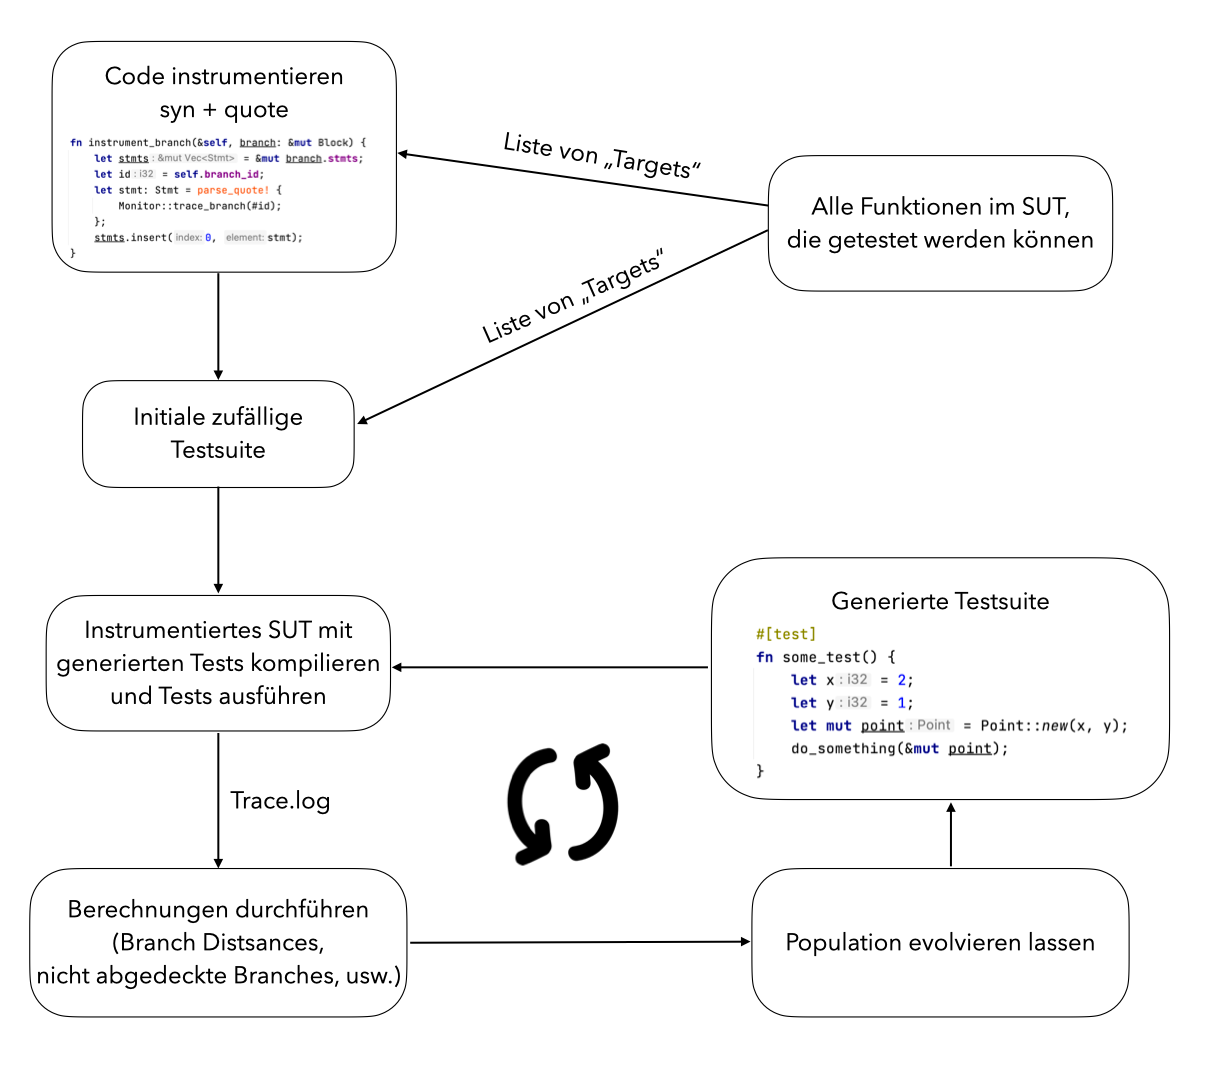
\includegraphics[width=\textwidth]{testify-overview}
\label{fig:testify-overview}
\end{figure}
\subsection{Testability Transformations}
\subsection{Instrumentation}
\subsection{Test Suite Optimization}
Figure~\cref{fig:testify-overview} illustrates the main steps in the Testify Tool: It starts by instrumenting the \ac{SUT} and inserting necessary statements to trace a programm execution. Then, a random test suite is generated based on the \ac{SUT} and evolved using evolutionary search towards a specified fitness goal. At the end, the test suite with the highest coverage is returned. 

\subsubsection{Problem representation}
Laut McMinn~\cite{McMinn_2004} sollte eine Enkodierung der Lösung so gewählt sein, dass ähnliche Lösungen ebenfalls \"Nachbarn\" im repräsentierten Suchraum sind. Dadurch kann die Suche leicht von einer zur ähnlichen Lösung durch einfache Modifikationen der Repräsentation fortgeführt werden. In genetischen Algorithmen für Testgenerierung repräsentiert ein Chromosom in einer Population typischerweise eine ganze Testuite~\cite{Fraser_2011, Campos2017}. Fraser und Arcuri schlagen folgendes zu Repräsentation der Lösung vor~\cite{Fraser_2011}: Eine Lösung ist hier eine Test Suite~$T$, die im Grunde ein Set von Unit Tests ist und für welchen gilt: Wenn~$|T| = n$, dann~$T = \{t_1, t_2, ... ,t_n\}$. Ein Unit Test ist demnach eine Sequenz von Statements bzw. Programmaufrufen, die Teile des \ac{SUT} ausführen, um ein gewisses Objective (bzw. Branch) zu erreichen und abzudecken. Da Programme in Rust nicht nur Prozeduren sind, sondern eine bestimmte, Klassen-ähnliche Struktur haben, muss dies ebenfalls berücksichtigt werden. In einem einfachen prozeduralen Programm müssten Tests nur Prozeduren mit bestimmten Input-Daten aufrufen, um eine hohe Coverage zu erreichen. Instanzen von Klassen und (in Rust) Klassen-ähnlichen Structs können jedoch Zustände haben, die entweder direkt oder per Methodenaufrufe geändert werden können. Der Kontrollflussgraph einer Methode kann vom inneren Zustand eines Objekts abhängig sein. Das heißt, dass eine gewisse Statementaufrufsequenz von Bedeutung sein kann, um eine hohe Branch Coverage zu erreichen. Für die Generierung von Unit Tests mit einem genetischen Algorithmus werden in dieser Arbeit bereits bekannte Ideen für die Repräsentationen von genetischen Lösungen umgesetzt~\cite{Fraser2012,Tonella2004,Arcuri2008}.

Somit ist jedes Statement in einem Test ein Wert~$v(s_i)$, welcher von einem der fünf folgenden Typen~$\tau(v(s_i))$ sein kann:
\begin{itemize} 
	\item \textbf{Primitive Statements} repräsentieren numerische Variablen, z. B. \lstinline{let v = 42}. Der Wert und Typ des Statements werden von der primitiven Variable bestimmt. 
	\item \textbf{Konstruktor-Statements} generieren neue Instanzen eines gegebenen Structs, z. B. \lstinline{let s = SomeStruct::new()}. Der Wert und Typ des Statements werden vom Struct bestimmt. Ein Konstruktor kann Parameter haben, denen ebenso der Wert aus dem Set~$\{v(s_k) | 0 \leq k < i\}$ zugewiesen wird.
	\item \textbf{Attribut-Statements} greifen auf die public member variables von Objekten, z. B. \lstinline{let b = a.x}. Der Wert und Typ eines Attribut-Statements sind von der member variable abhängig. Die Quelle der member variable, also~\lstinline{a}, muss ebenso Teil des Sets~$\{v(s_k) | 0 \leq k < i\}$ sein. 
	\item \textbf{Methoden-Statements} führen Methoden auf Objekten aus oder rufen statische Methoden auf, z. B. \lstinline{let b = a.len()}. Hier wieder, das Quellobjekt und jegliche Parameter der Methode müssen Teil des Sets~$\{v(s_k) | 0 \leq k < i\}$ sein. Der Wert und Typ des Statements werden vom Return-Wert der Methode bestimmt. 
	\item \textbf{Funktionen-Statements} führen lose bzw. frei stehende Funktionen aus, z. B. \lstinline{let a = do_something()}. Die möglichen Parameter einer solchen Funktion müssen Teil des Sets~$\{v(s_k) | 0 \leq k < i\}$ sein. Der Wert und Typ des Statements werden vom Return-Wert der Funktion bestimmt. 
\end{itemize}

Die Sammlung von verfügbaren Structs, deren Konstruktoren, Methoden, Felder und frei stehende Funktionen sind ein sogenannter Test Cluster~\cite{Fraser_2011}. Die Größe einer Test Suite sowie einzelner Tests ist dabei dynamisch und kann sich (fast) beliebig verändern. Da für die meisten generierten Tests keine Testorakel zur Verfügung stehen werden, soll die Größe der Test Suite sowie der einzelnen Tests eine Obergrenze haben (kein Mensch möchte tausende Zeilen lange Tests durchlesen, um am Ende eine passende Assertion zu überlegen). 

Jedes Statement, welches nicht den default Rückgabewert~\lstinline{()} hat, welcher ähnlich zu~\lstinline{void} in C-ähnlichen Sprachen ist, definiert eine neue Variable. Ein generierter Test kann jedoch nicht beliebig aus den oben genannten Bausteinen zusammengesetzt werden. Er unterliegt den gleichen Constraints, wie reguläre Rust Programme, die vom Compiler überprüft werden~\cite{Tonella2004}. Diese sind: \todo{Weitere?}
\begin{enumerate}
    \item Variablen müssen immer definiert und initialisiert sein, bevor sie benutzt werden (als Argumente von Funktionen und Methoden oder als Target eines Methodenaufrufs)
    \item Eine konsumierte Variable darf nach dem konsumierenden Statement nicht noch mal verwendet werden
    \item Eine von einer Funktion oder Methode als \textit{mutable} ausgeliehe Variable muss beim Aufruf der Funktion oder Methode als solche übergegen werden
\end{enumerate}
Konstruktoren, Methoden, Funktionen und Felder in einem Test sind nicht nur auf die Teile des Moduls unterm Test begrenzt, da für die Definition einiger Argumente komplexe Sequenzen von Aufrufen notwendig sein könnten~\cite{Fraser2012}. 

Fraser und Zeller~\cite{Fraser2012} beschreiben in ihrer Arbeit zum Mutations-basiertem Generieren von Tests für Java Klassen ein abstraktes Konstrukt, welches die Modellierung und Aufbau eines Unit Tests leicht veranschaulicht. Sei~$parameters(M)$ eine Funktion, die eine Liste von Datentypen der Parameter einer Methode oder Funktion~$M$ zurückgibt, einschließlich des Aufrufers im Falle einer nicht-statischen Methode. Des Weiteren, sei~$classes(t)$ eine Funktion, die den Set von Datentypen zurückgibt, dessen Objekte in einem Test~$t$ bereits instanziert wurden. Eine Funktion oder eine Methode ist ein Generator eines Datentyps~$C$ wenn sie einen Rückgabewert vom Typ~$C$ haben. Außerdem ist jeder Konstruktor eines Structs vom Typ~$C$ ebenfalls ein Generator von~$C$. Sei~$generators(M,C)$ eine Funktion, die den Set von Generatoren für den Datentyp~$C$ aus dem Set von Methoden und Funktionen~$M$ zurückgibt. 

\begin{algorithm}[t]
\caption{$GenTest(M, l)$}\label{alg:random-generation-of-a-test}
\begin{algorithmic}
\Input
  \Desc{$M$}{Set of all method, constructors and functions}
  \Desc{$l$}{Desired length of a test case}
\EndInput
\Output
  \Desc{$t$}{Randomly generated test}
\EndOutput    
\State{$t \gets \langle\rangle$}
\State{$s \gets$ randomly select an element from M}


\For{$p \in parameters(s)$}
  \State{$t \gets GenObject(p, \{\}, M, t)$}
\EndFor
\State{$t \gets t.s$}

\While{$\left|t\right| < l$}
  \State{$c \gets$ randomly select datatype in $classes(t)$}
  \State{$M' \gets \{m | m \in M \wedge c \in parameters(m)\}$}
  \State{$s \gets$ randomly select method or function from $M'$}
  \For{$p \in parameters(s)$}
    \If{$\neg(p \in classes(t))$}
      \State{$t \gets GenObject(p, \{\}, M, t)$}
    \EndIf
  \EndFor
  \State{$s \gets$ set parameters of $s$ to values from $t$}
  \State{$t \gets t.s$}
\EndWhile
\State \Return $t$
\end{algorithmic}
\end{algorithm}


Die initiale Population wird zufällig generiert, wie im Algorithmus~\labelcref{alg:random-generation-of-a-test} dargestellt. Bevor die Tests generiert werden, werden alle verfügbaren Methoden, Konstruktoren und Funktionen, sowie Attribute von Structs statisch extrahiert. Bei einem zufällig generierten Test wird daraus ein zufälliger Aufruf eingefügt. Die evtl. notwendigen Argumente (inklusive des Aufrufers) werden dabei ebenfalls generiert. Dafür werden entsprechende Aufrufe, die Rückgabewerte von passenden Datentypen haben, rekursiv eingefügt (Algorithmus~\labelcref{alg:random-generation-of-args}), wenn im Test Case nicht bereits Instanzen eines solchen Datentyps definiert sind. Während der Suche werden die Datentypen, die zu instanziieren bereits versucht wird, gemerkt, um unendliche Rekursionen zu vermeiden. Laut den Algorithmen~\labelcref{alg:random-generation-of-a-test} und~\labelcref{alg:random-generation-of-args} werden neue Objekte nur dann generiert, wenn sie nicht im Test bereits existieren. Fraser und Zeller~\cite{Fraser2012} schlagen jedoch vor, bestehende Objekte nur mit einer gewissen Wahrscheinlichkeit wiederzuverwenden, um Diversität in generierten Test Cases zu erhöhen. In ihren Experimenten haben sie festgestellt, dass eine Wahrscheinlichkeit von 90\% Prozent am effektivsten ist. Rusts affines Typsystem macht eine Wiederverwendung von bereits definierten Objekten komplizierter, da die Information, in welchen Aufrufen eine bestimmte Instanz auf welche Weise verwendet wurde (ausgeliehen oder konsumiert) ebenfalls mitgeführt werden muss. Das heißt, dass ein bereits definiertes Objekt nur dann von einem neu eingefügten Statement~$s$ verwendet werden darf, wenn es als frei verwendbar markiert ist und von keinem anderen Statement verwendet wird, das nach~$s$ kommt. Genauer werden die Regeln folgenderweise definiert: Sei~$t$ ein Test Case und $pos(s)$ eine Funktion, die die Position eines Statements~$s$ in der Sequenz von~$t$ zurückgibt. Sei~$o$ ein Objekt von einem Datentyp~$c$, das von einem Statement~$gen$ definiert wird. Ein neues Statement~$s'$ wird eingefügt, welches~$o$ verwendet. Es gilt für die Positionen:~$pos(gen) < pos(s')$. Außerdem gilt:
\begin{itemize}
    \item Wenn~$o$ von keinem Statement~$s \in t$ verwendet wird, darf~$o$ von~$s'$ konsumiert und ausgeliehen werden. 
    \item Wenn~$o$ von einem Statement~$s \in t$ ausgeliehen wird, darf~$o$ von~$s'$ an der Position~$p_{borrow}$ mit ~$pos(gen) < p_{borrow}$ ebenfalls ausgeliehen oder an der Position~$p_{consume}$ mit~$pos(s) < p_{consume} < \left|t\right|$ konsumiert werden. 
    \item Wenn~$o$ von einem Statement~$s \in t$ konsumiert wird, darf~$o$ von~$s'$ an der Position~$p_{borrow}$ mit~$pos(gen) < p_{borrow} < pos(s)$ ausgeliehen werden. 
\end{itemize}
Das Ganze wird mit Hilfe eines Data Dependence Graphen realisiert, in dem jedes Statement bzw. ein definiertes Objekt die Rolle eines Knoten hat und Beziehungen wie z. B. \textit{Consumes} oder \textit{Borrows} zwischen Statements und ihren Argumenten notiert werden können. 


Fraser und Zeller schlagen ebenfalls vor, wenn sich eine zufällige Generierung als schwierig erweist, kann Algorithmus~\labelcref{alg:random-generation-of-args} in eine umfassende Suche mit Backtracking umgewandelt werden. Auch wenn der Suchraum groß ist, sei das gar kein so großes Problem, da Teilsequenzen zur Generierung von Instanzen wiederverwendet werden können. Die Test Cases werden so lange auf diese Weise produziert, bis die gewünschte Größe der Population erreicht ist. 



\begin{algorithm}[t]
\caption{$GenObject(c, G, M, t)$}\label{alg:random-generation-of-args}
\begin{algorithmic}
\Input
  \Desc{$c$}{Datatype of desired object}
  \Desc{$G$}{Set of datatypes already attempting to generate}
  \Desc{$M$}{Set of all method, constructors and functions}
  \Desc{$t$}{Test case}
\EndInput
\Output
  \Desc{$t$}{Test case extended with an instance of $c$}
\EndOutput    
\State{$M' \gets generators(M, c)$}
\State{$s \gets$ randomly select an element from M'}

\For{$c \in parameters(s)$}
  \If{$\neg(c \in classes(t))$}
    \State{$t \gets GenObject(c, G, M, t)$}
  \EndIf
\EndFor
\State{$s \gets$ set parameters of $s$ to values from $t$}
\State{$t \gets t.s$}
\State \Return $t$
\end{algorithmic}
\end{algorithm}

\subsubsection{Bloat Control}
Hier wird beschrieben, wie man verhindern kann, dass die Größe der Test Suite und einzelner Tests ausartet. Fraser und Arcuri~\cite{Fraser_2011} haben ein paar Gedanken dazu. 

\subsubsection{Search Operators}
Suchoperatoren wie Crossover, Mutation und Random Test Case werden hier beschrieben. Natürlich haben auch Fraser und Arcuri~\cite{Fraser_2011} eine ausführliche Beschreibung der Funktionsweise. 

\subsubsection{Mutation}
Chromosome werden hier in ihrer ''natürlichen'' Weise repräsentiert, also nicht in der Binärform. Das heißt für einen Test Case, dass er aus einer Sequenz von Statements besteht. Diese können auf verschiede Weisen mutiert werden: 

\textbf{Insert a method or function invocation}: Ein neuer Methodenaufruf wird dem Test Case hinzugefügt. Die von der Methode benötigten Argumente werden ebenfalls, wenn nötig initialisiert, und hinzugefügt. Eine Variable wird zufällig ausgewählt, deren Methode aufgerufen werden soll, oder ein neues Objekt wird zuvor erstellt, mit einem Datentypen, welcher im jeweiligen Test bereits verwendet wurde~\cite{Fraser2012}. Der Aufruf wird zufällig zwischen dem Initialisieren des Objects und dem Aufruf der \ac{MUT} eingefügt (falls man überhaupt von einem festgesetzten MUT, also bottom-up, ausgeht). Es können auch mehrere Methodenaufrufe wiederholt eingesetzt werden, wobei dies mit der Wahrscheinlichkeit~$p(n) = 0.5^n$ passiert, wo $n$ die Anzahl von bisher eingefügten Aufrufen ist. Das heißt, dass nach jedem Einsetzten eine zufällige Entscheidung getroffen wird, ob die Mutation wiederholt werden soll~\cite{Tonella2004}.
\begin{lstlisting}[language=Java, caption=, label=lst:mutation-invocation-insertion]
let a = A::new();
a.m(10, 5);

// wird zu 
let a = A::new();
let b = B::new();
a.f(b);
a.m(10, 5);
\end{lstlisting}

\textbf{Delete a method or function invocation}: Einige Methodenaufrufe können zufällig aus einem Test Case gelöscht werden. Werte, die dadurch im Test Case nicht mehr verwendet werden, werden ebenso gelöscht. Falls das gelöschte Statement~$s$ einen Rückgabewert hatte, welcher von einem anderen Statement~$s'$ verwendet wird, muss~$s'$ entweder ebenfalls gelöscht werden oder das entsprechende Argument durch ein anderes, im Test bereits definiertes Objekt des gleichen Datentyps ersetzt werden~\cite{Fraser2012}.
\begin{lstlisting}[language=Java, caption=, label=lst:mutation-invocation-removal]
let a = A::new();
let b = B::new();
a.f(b);
a.m(10, 5);

// wird zu 
let a = A::new();
a.m(10, 5);
\end{lstlisting}
Der Aufruf von \lstinline{a.f(b)} wurde zufällig zum Löschen ausgewählt. Da es die einzige Stelle war, an der \lstinline{b} verwendet wurde, wurde es ebenfalls gelöscht. Ähnlich wie das Einsetzen von Methodenaufrufen, kann dieser Operator mit der Wahrscheinlichkeit~$p(n) = 0.5^n$ wiederholt angewendet werden, wobei $n$ die Anzahl von gelöschten Statements ist. 

\textbf{Modify an existing statement}: Eine der folgenden Veränderungen wird angewendet~\cite{Fraser2012}:
\begin{itemize}
  \item \textit{Change callee:} For a method call or field reference, change the source object.
  \item \textit{Change parameters:} Change one parameter of a method, constructor or function call to a different value or create a new value.
  \item \textit{Change method/constructor/function:} Replace a call with a different one with an identical return type.
  \item \textit{Change field:} Replace a primitive value with a different primitive value of the same type.
\end{itemize}
\begin{lstlisting}[language=Java, caption=, label=lst:mutation-input-value]
let a = A::new();
a.m(10, 5);

// wird zu 
let a = A::new();
a.m(20, 5);
\end{lstlisting}

\subsubsection{Crossover}
Die einfachste Art von Crossover ist der One-Point-Crossover, so wie er in~\cref{sec:background-crossover} beschrieben ist. Die Chromosome werden hier jedoch in der natürlichen Art repräsentiert, als Sequenz von Statements, was dazu führt, dass beim Aufteilen und Durchtauschen von Köpfen eines Paars von Chromosomen auf die Abhängigkeiten der Statements geachtet werden muss. Tonella~\cite{Tonella2004} schlägt zwei Alternativen vor:
\begin{itemize}
    \item Fehlende Abhängigkeiten von Statements können wie beim Mutationsoperator durch das Generieren ergänzt werden. \todo{Beispiel} Sollten bestimmte Definitionen dadurch überflüssig werden, dass ihre spätere Benutzung durch Rekombination in ein anderes Choromosom geschoben wurde, können diese gelöscht werden. 
    \item Abhängigkeiten von einem durch Rekombination verschobenen Teil eines Chromosoms werden unabhängig vom Crossover-Point ebenfalls in ein anderes Chromosom geschoben, sofern diese im ursprünglichen Chromosom nicht mehr benötigt werden. \todo{Beispiel}
\end{itemize}

\subsubsection{Dependencies}
Hat man beispielsweise ein Rust Programm wie in Listing~\ref{lst:example-rust-program}, welches raus einem Struct für Rechtecke und einem Struct, welcher Operationen auf dem Rechteck durchführt (was nicht ganz der guten Sitten des Software Engineering entspricht, daher sollte ein besseres Beispiel hergenommen werden). 

\begin{lstlisting}[language=Java, caption=Ein Beispiel für ein Rust Program, label=lst:example-rust-program]
struct Rectangle {
    width: u64,
    height: u64,
}

impl Rectangle {
    pub fn new(width: u64, height: u64) -> Self {
        Rectangle { width, height }
    }
    pub fn width(&self) -> u64 {
        self.width
    }
}

struct Calculator {}

impl Calculator {
    pub fn new() -> Self {
        Calculator {}
    }
    pub fn area_by_value(&self, r: Rectangle) -> f64 {
        r.height as f64 * r.width as f64
    }
}
\end{lstlisting}
Ein Beispiel Testcase für das Program kann wie im Listing~\ref{lst:example-testcase} aussehen. Dabei wird ein Rechteck mit einer bestimmten Länge und Breite erstellt und vom Calculator konsumiert, um die Fläche des Rechtecks zu bestimmen. Das affine Typsystem von Rust erlaubt es nicht,\todo{Verschiedene Typsysteme in einer kleinen Übersicht erklären?} dass die Variable~\lstinline{calculator_0} noch mal verwendet wird. Es kann also nach dem Statement in der Zeile 4 weder auf die Attribute von dem Recheck zugegriffen werden, noch kann das Rechteck als Argument für weitere Aufrufe dienen. 
\begin{lstlisting}[language=Java, caption=Ein Beispiel Testcase, generiert für das Program im Listing~\ref{lst:example-rust-program}, label=lst:example-testcase]
let mut rectangle_0 = Rectangle::new(205u8, 166u8);
let u64_0 = rectangle_3.width();
let mut calculator_0 = Calculator::new();
let f64_4 = areacalculator_0.area_by_value(rectangle_0);
\end{lstlisting}
Die im Testcase aus dem Listing~\ref{lst:example-testcase} können mit einer Art von Data-Dependence-Graph wie in Figure~\ref{fig:ddg-example}.

\begin{figure}[h]
\caption{Data-Dependence-Graph für den Testcase aus dem Listing~\ref{lst:example-testcase}}
\centering
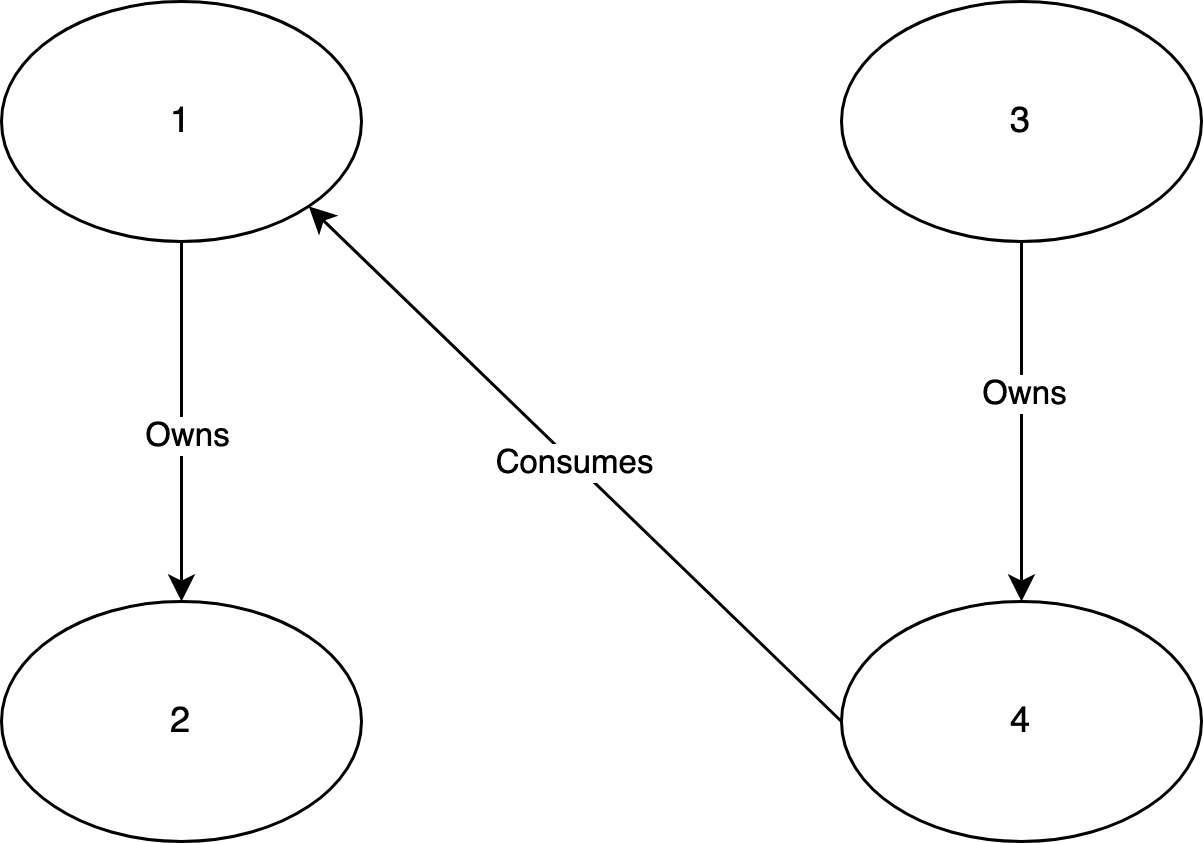
\includegraphics[width=\textwidth]{DDG}
\label{fig:ddg-example}
\end{figure}

\subsubsection{Fitness Function}
Um die Selektion von Parents für die nachkommende Generationen besser guiden zu können, werden alle Individuen in einer Population nach ihrer Fitness ausgewertet. Eine gute Fitnessfunktion ist sehr wichtig bei der Suche nach Lösungen. Lösungen, die in einer bestimmten Weise \"besser\" als andere sind, sollen mit besseren Fitnesswerten belohnt werden. Was auch immer eine bessere Fitness ist, eine höhere oder niedrigere Fitness hängt davon ab, ob die Suchstrategie versucht, die Fitnessfunktion zu maximieren oder zu minimieren~\cite{McMinn_2004}. Dieser Ansatz wird sich voraussichtlich auf Branch Coverage konzentieren. EvoSuite instrumentiert in der originalen Implementierung Java SUT auf Bytecode-Level und im Bytecode werden alle Loops usw. in die einfachen if-Verzweigungen überführt. Das Ziel ist es, die optimale Lösung zu finden, d. h. eine Test Suite, die möglichst hohe Branch-Coverage hat. Gleichzeitig soll es aber keine andere Testsuite geben, die bei gleicher Branch-Coverage kleiner ist bzw. kleinere Tests enthält. Einige Branches, sogenannte infeasible Branches, können evtl. gar nicht abgedeckt werden, entweder aufgrund der limitierten Repräsentation der Lösung oder weil es keine passenden Inputs existieren. Somit werden solche Tests bevorzugt bei der Evolvierung bevorzugt, die eine höhere Fitness bzgl. der Branch-Coverage haben. Bei zwei Tests mit der gleichen Coverage wird der kürzere bevorzugt. 

Um die Suche voranzutreiben, können verschiedene Heuristiken verwendet werden. \todo{Welche gibt es überhaupt?} Eine der weitverbreitesten ist Branch Distance. McMinn~\cite{McMinn_2004} beschreibt eine Sammlung von Regeln, die rekursiv angewendet werden können, um Distanz bei allen möglichen Prädikaten zu berechnen. Wenn die Ausführung des \ac{SUT} bei gegebenen Inputdaten in einem bestimmten Branch landet, so kann eine lokale Suche angewendet werden. Es wird mit Hilfe einer lokalen Fitnessfunktion abgeleitet, wie nah das Prädikat zum Auswerten zu \lstinline{true} ist. Zum Beispiel, bei einem Prädikat~\lstinline{x >= 10} und~\lstinline{x = 5} (während der Ausführung) wird der \lstinline{false} Branch getroffen. Die Distanz zum \lstinline{true} Branch beträge somit~$10 - 5 + k$ mit~$k \geq 1$. Dabei wird jedes Prädikat im \ac{SUT} instrumentiert, um die Distanzen zu anderen Branches während der Ausführung des \ac{SUT} zu tracen. Die Branch-Distanz muss noch normalisiert werden (je nach Werten kann es schnell zu Extremen kommen). Arcuri~\cite{Arcuri_2011} beschreibt in seiner Arbeit, welchen Einfluss die Normalisierung der Branch-Distanz auf die Effektivität einer such-basierten Testgenerierung hat. 

\subsection{Usability}
EvoSuite scheint sehr auf Usability ausgerichtet zu sein, zum Beispiel gibt es ein Eclipse Plugin, welches man per Click zum Generieren von Tests für das offene Projekt benutzen kann. Außerdem, da SBST mit Iterationen arbeitet, kann man die Ausführung jederzeit beenden und die bisher besten Ergebnisse zurück geben~\cite{Harman2015}. Das obere Limit für die Ausführungszeit von generierten Tests ist in diesem Kontext von Bedeutung. 
\section{Evaluation}
\subsection{Setup}
\subsection{Threats to Validity}
\subsection{Code Coverage Comparison with Manually Written Tests}
\subsection{Code Coverage Comparison with Other Tools}


\section{Conclusion}

\section{Future Work}

\appendix
\chapter{Acronyms}
\begin{acronym}
	\acro{SUT}{System Under Test}
	\acro{CUT}{Class Under Test}
	\acro{MUT}{Method Under Test}
	\acro{SMT}{Satisfiability Modulo Theories}
	\acro{GA}{Genetic Algorithm}
	\acro{EA}{Evolutionary Algorithm}
	\acro{MOSA}{Many-Objective Sorting Algorithm}
	\acro{DynaMOSA}{Many-Objective Sorting Algorithm with Dynamic target selection}
	\acro{WS}{Whole Suite}
	\acro{WSA}{Whole Suite with Archive}
	\acro{SBST}{Search-based Software Testing}
	\acro{SBSE}{Search-based Software Engineering}
	\acro{ATP}{Automated Theorem Prover}
	\acro{DSE}{Dynamic Symbolic Execution}
	\acro{IR}{Intermediate Representation}
	\acro{MOA}{Multi- and Many-Objective Algorithm}
	\acro{DDG}{Data Dependence Graph}
	\acro{HIR}{High-level Intermediate Representation}
	\acro{THIR}{Typed HIR}
	\acro{MIR}{Mid-level Intermediate Representation}
	\acro{AST}{Abstract Syntax Tree}
	\acro{CFG}{Control Flow Graph}
	\acro{CDG}{Control Dependence Graph}
	\acro{API}{Application Programming Interface}
	\acro{NSGA-II}{Non-dominated Sorting Genetic Algorithm II}
	\acro{TCP}{Transmission Control Protocol}
	\acro{SSA}{Static Single Assignment}
\end{acronym}


\bibliographystyle{unsrt}
\bibliography{bibliography}
%\nocite*{}
\end{document}